\documentclass[a4paper]{ctexart}

\usepackage{graphicx}
\usepackage[hmargin=1.25in,vmargin=1in]{geometry}
\usepackage[x11names]{xcolor} %must before tikz, x11names defines RoyalBlue3
\usepackage[bookmarksnumbered,unicode, pdfborder=1,breaklinks,colorlinks,linkcolor=RoyalBlue3,urlcolor=blue]{hyperref}
\usepackage{tabularx}

\usepackage{fancyhdr}

\pagestyle{fancy}
\fancyhf{}
\cfoot{\thepage}
\rhead{\tiny{中标麒麟服务器操作系统~V7.0(aarch64~版)-DVD光盘安装手册-V1.0\\CS2C-NSHW-UM-DVDInstall-V1.0}}
\lhead{
\includegraphics[width=3.5cm]{ns7/cs2c-logo}}
\renewcommand{\headrulewidth}{0.4pt}

\usepackage[raggedright]{titlesec}

%\titleformat*{\section}{\Large\bf\raggedright}

%行距
%\renewcommand{\baselinestretch}{1.25}
\linespread{1.5}

%段落
%\setlength{\parindent}{em}

\begin{document}

\pagenumbering{Roman}
%\pdfbookmark{标题页}{title}
\thispagestyle{empty}

\vspace*{\stretch{0.2}}
\noindent\begin{minipage}{\textwidth}
\begin{flushright}
	
\includegraphics[scale=1.0]{ns7/cs2c-short-logo}
\end{flushright}
\end{minipage}

\vfill
\noindent\begin{minipage}{\textwidth}
\centering
{\LARGE \bfseries 中标麒麟服务器操作系统~V7.0~(aarch64版)}
\noindent\rule[1.5ex]{\textwidth}{1pt}\\[1ex]
\hfill 
{\Large \bfseries DVD光盘安装手册}
\end{minipage}

\vfill
\noindent\rlap{%
  \begin{minipage}{\textwidth}
  \linespread{2.5}\selectfont\raggedright
  中标软件有限公司\\
  上海市徐汇区番禺路~1028~号数娱大厦~10~层(200030)\\
  北京市海淀区北四环西路~9~号银谷大厦~20~层(100190)\\
  广州市天河北路~898~号信源大厦~16~层~1604~室(510898)\\
  \end{minipage}%
}

\vspace*{\stretch{0.2}}
\newpage

%\thispagestyle{empty}
%\begin{quote}\footnotesize
%    Copyright \copyright{}  2016  Louis Stuart. \\
%    Permission is granted to copy, distribute and/or modify this document
%    under the terms of the GNU Free Documentation License, Version 1.3
%    or any later version published by the Free Software Foundation;
%    with no Invariant Sections, no Front-Cover Texts, and no Back-Cover Texts.
%    A copy of the license is included in the section entitled ``GNU
%    Free Documentation License''.
%\end{quote}

\titleformat*{\section}{\Large\bfseries\centering}

\section*{版本说明}
\vspace*{1.5ex}
\begin{tabularx}{36em}%
{|*{4}{>{\centering\arraybackslash}X|}}\hline

\bfseries 日期 & \bfseries 版本号 & \bfseries 发布说明 & \bfseries 编写者 \\ \hline
2016-07-11 & V1.0 & 发布稿 & 张超  \\ \hline
& & &  \\ \hline
& & &  \\ \hline
& & &  \\ \hline
& & &  \\ \hline
& & &  \\ \hline
& & &  \\ \hline
& & &  \\ \hline
& & &  \\ \hline
& & &  \\ \hline
& & &  \\ \hline
& & &  \\ \hline
& & &  \\ \hline
& & &  \\ \hline
& & &  \\ \hline
& & &  \\ \hline
& & &  \\ \hline
& & &  \\ \hline
& & &  \\ \hline
& & &  \\ \hline
& & &  \\ \hline
& & &  \\ \hline
& & &  \\ \hline
& & &  \\ \hline
& & &  \\ \hline
& & &  \\ \hline
& & &  \\ \hline
& & &  \\ \hline
& & &  \\ \hline
& & &  \\ \hline
\end{tabularx}
\vfill
\clearpage

% 目录
\titleformat*{\section}{\Large\bfseries\centering}
\tableofcontents
\clearpage

\pagenumbering{arabic}
\titleformat*{\section}{\Large\bfseries\raggedright}
\section{引言}
\subsection{编写目的}
中标麒麟服务器操作系统~V7.0~(~aarch64~版)拥有全新设计的用户界面、统一的应用程序及工具入口、简单实用的各类软件,使整个操作系统更加高效、易用,再加上其良好的兼容性,必将给您带来前所未有的使用体验。为方便使用者更加轻松地体验操作系统,现整理安装手册供用户快速了解系统的安装过程。

本说明书的预期读者为项目经理、项目组全体开发人员和普通用户。

\subsection{背景}
本产品为通用操作系统,相关背景信息如下: \par
产品名称:中标麒麟服务器操作系统~V7.0~(~aarch64~版) \par
产品研发代号:NSHW \par
产品版本号:V7.0 \par
任务提出者:中标软件有限公司专用~OS~事业本部产品部 \par
任务开发者:中标软件有限公司专用~OS~事业本部研发部 \par
目标用户:通用领域用户 

\subsection{运行平台}
HW Taishan~服务器

\section{DVD~光盘镜像安装}
\subsection{安装前准备}
\begin{enumerate}
\item 刻录中标麒麟服务器操作系统~V7.0~系统镜像~DVD~光盘;
\item 适用于~HW~服务器的低电压外置光驱。
\end{enumerate}

\subsection{安装系统}
将系统镜像置入外置光驱内,并将外置光驱正确连接到~HW~服务器。开启电源,启动服务器。

根据启动信息提示按“F4”或者“Delete”进入~BIOS~设置\footnote{期间有验证界面,请根据提示输入正确的验证信息},进入~BIOS~设置界面后通过键盘上的左右方向键调整到~Boot~页,此时可以看到“EFI USB Device *”及光驱信息那一项,选择并按\textbf{~Enter~}确认,等待系统系统启动到安装菜单项界面,该界面上会有默认已选择的“Install NeoKylin Server 7.0”字符选项,按\textbf{~Enter~}确认,即可开始安装。

首先显示的界面如图~\ref{fig:welcome-install}~为安装欢迎界面,在该界面可以通过鼠标或者键盘上的方向键及\textbf{~Tab~}键进行安装过程语言的选择,默认选择为“中文”。

\begin{figure}[htp]
	\centering
	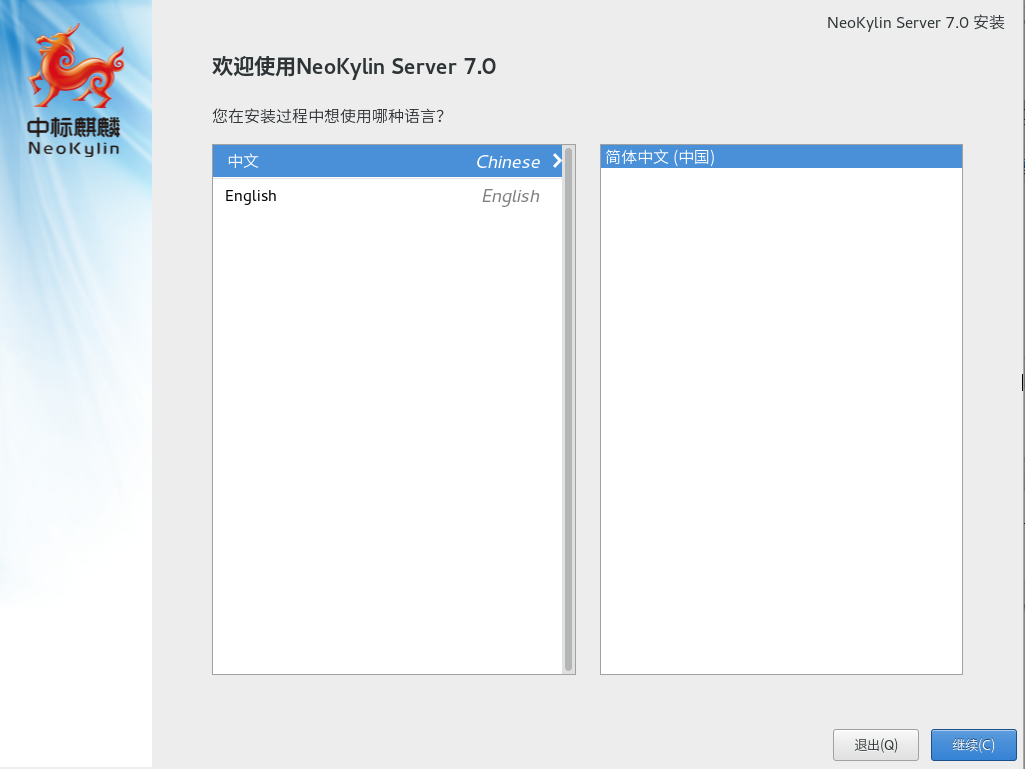
\includegraphics[width=11cm]{ns7/welcome-installation}
	\caption{安装欢迎界面}\label{fig:welcome-install}
\end{figure}

点击\textbf{继续},进入安装信息摘要界面。在刚进入安装信息摘要界面时后台会自动配置相关选项,此时有些选项会处于“disable”状态,用户不可以点击进入调节,当自动配置完成后选项会自动置为“enable”状态,此时用户可以点击进入设置。默认这些配置都会自动完成,对于有些不能自动配置完成的,界面下方会有黄色条状提示,用户可以根据提示调节相关配置选项。

\begin{figure}[htp]
	\centering
	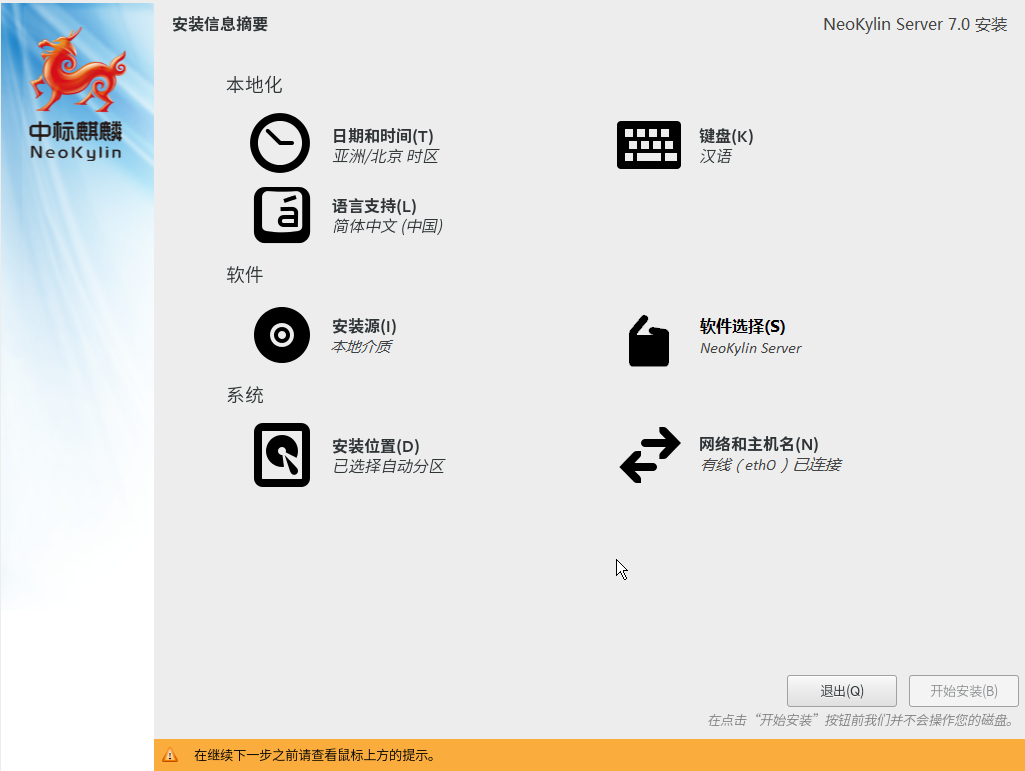
\includegraphics[width=10.5cm]{ns7/set-installation-info}
	\caption{安装信息摘要}\label{fig:set-installation-info}
\end{figure}

图~\ref{fig:set-installation-info}~界面所有需要设置的选项在没有正确配置前,右下角的\textbf{开始安装}将一直处于“disable”状态。

如果后台可以自动配置完成,则\textbf{开始安装}按钮将会处于“enable”状态,如图~\ref{fig:installaiton-info-complete}~。此时如果自动化配置能满足用户需求则直接点击\textbf{开始安装},就可以进行下一步,如图~\ref{fig:installation-progress}~。

\begin{figure}[htp]
	\centering
	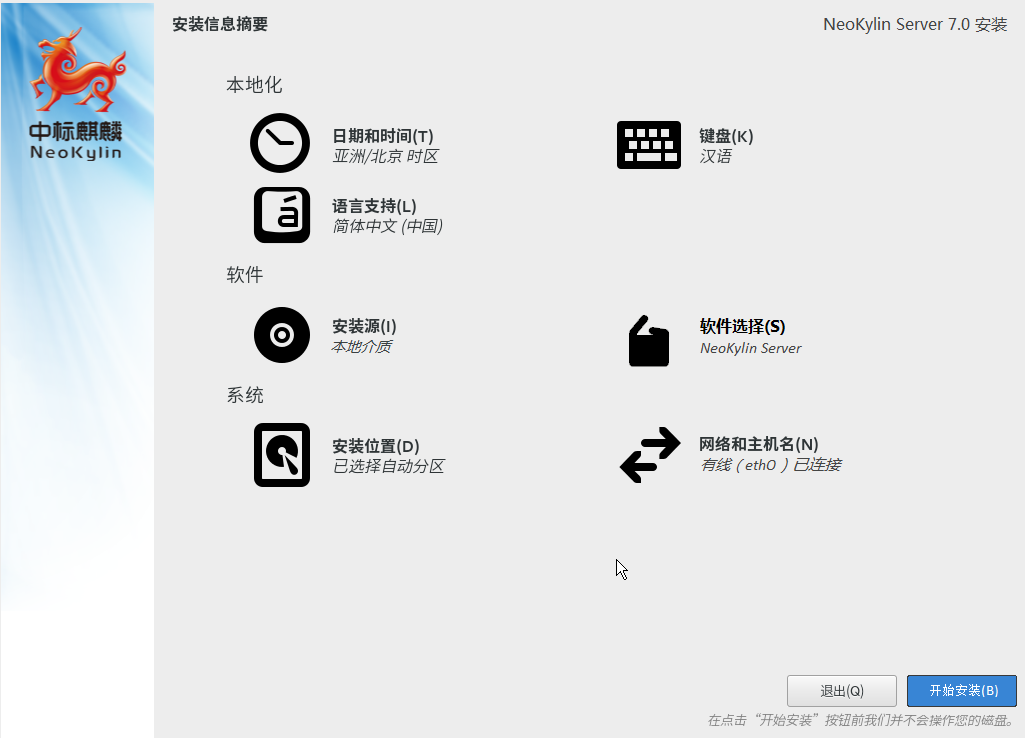
\includegraphics[width=10.5cm]{ns7/installation-info-complete}
	\caption{安装信息摘要设置完成}\label{fig:installaiton-info-complete}
\end{figure}


一般情况下,如果用户需要对分区进行自定义设置,则需要点击图~\ref{fig:set-installation-info}~“系统”-“安装位置”选项进行调整,如图~\ref{fig:partation-custom}~。
	
\begin{figure}[htp]
	\centering
	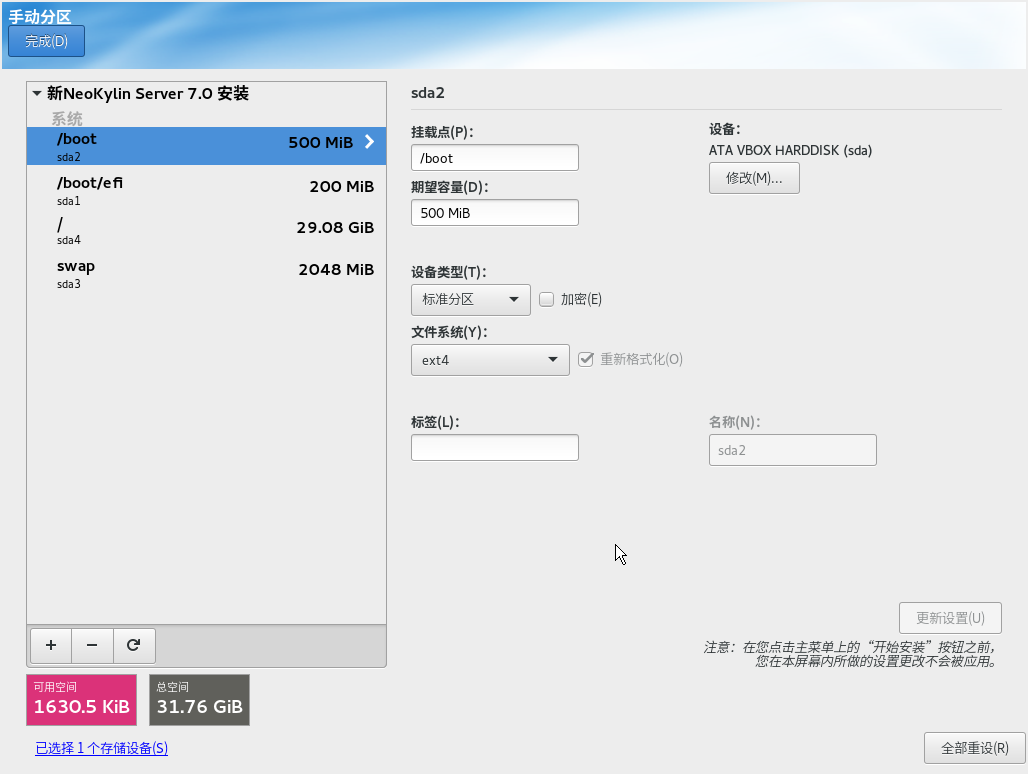
\includegraphics[width=10.5cm]{ns7/partation-custom}
	\caption{手动分区}\label{fig:partation-custom}
\end{figure}
 
用户可以通过左侧的\textbf{“+”“-”}进行分区的删减,可以通过右侧的输入框对各个分区进行大小的配置。如果分区配置不合适将会在界面下有黄色条状提示,用户可以根据提示信息重新调整分区状态,也可以通过右下角\textbf{全部重设}按钮进行恢复,重新对分区进行调整。
分区设置完成后,双击左上角\textbf{完成},会弹出自定义分区确认窗口,如图~\ref{fig:partation-custom-confirm}~。
 
\begin{figure}[ht]
	\centering
	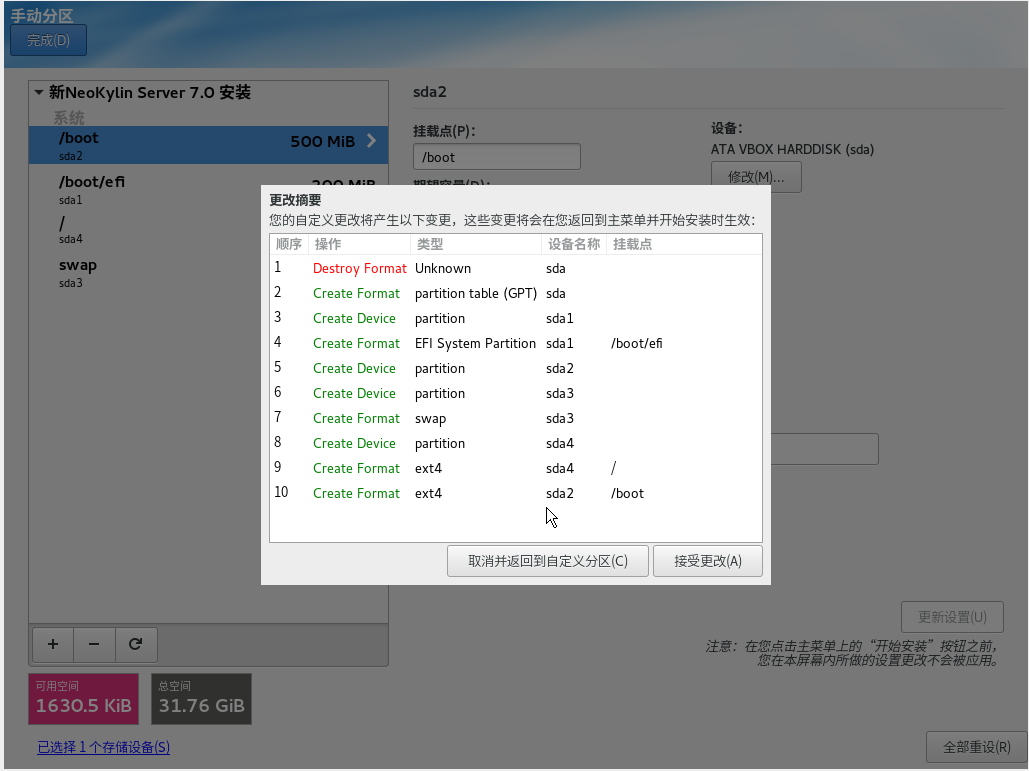
\includegraphics[width=10.5cm]{ns7/partation-custom-confirm}
	\caption{自定义分区}\label{fig:partation-custom-confirm}
\end{figure}
	  
点击\textbf{接受更改},将会返回到图~\ref{fig:installaiton-info-complete}~界面,此时\textbf{开始安装}按钮将会处于“enable”状态。
点击\textbf{开始安装}按钮进行系统安装,如图~\ref{fig:installation-progress}。

\begin{figure}[htp]
	\centering
	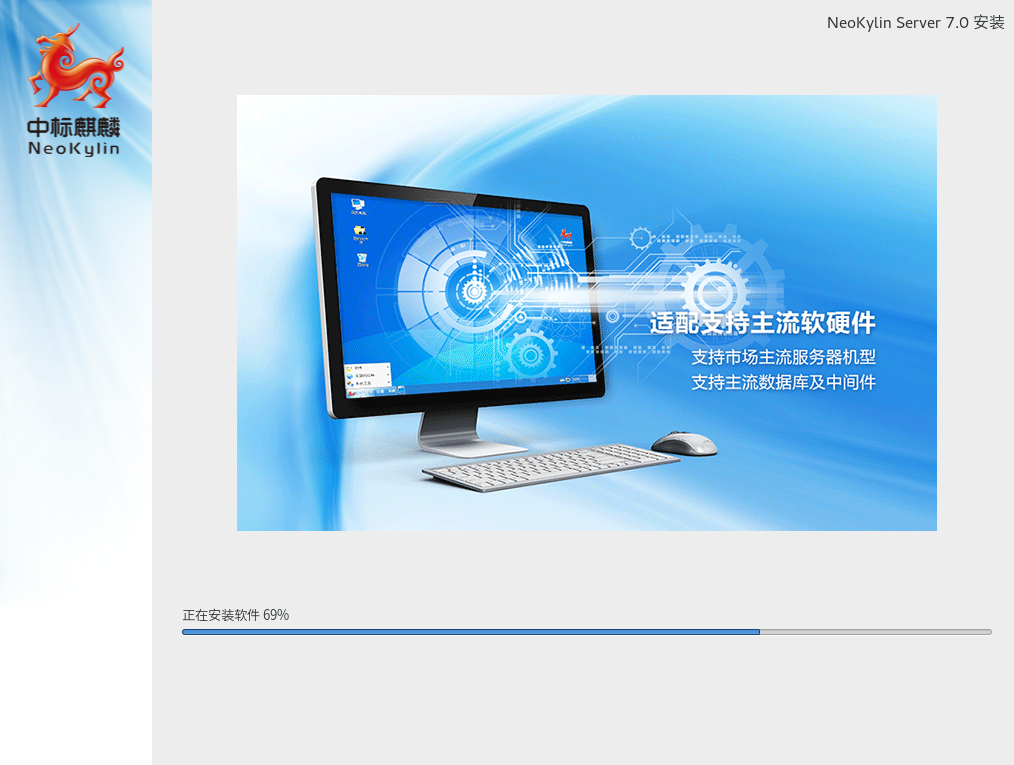
\includegraphics[width=10.5cm]{ns7/installation-progress}
	\caption{系统安装}\label{fig:installation-progress}
\end{figure} 

等待安装进度条完成,直到出现图~\ref{fig:installation-progress-complete}~中的\textbf{重启}按钮。此时,系统安装完成。

\clearpage

\begin{figure}[htp]
	\centering
	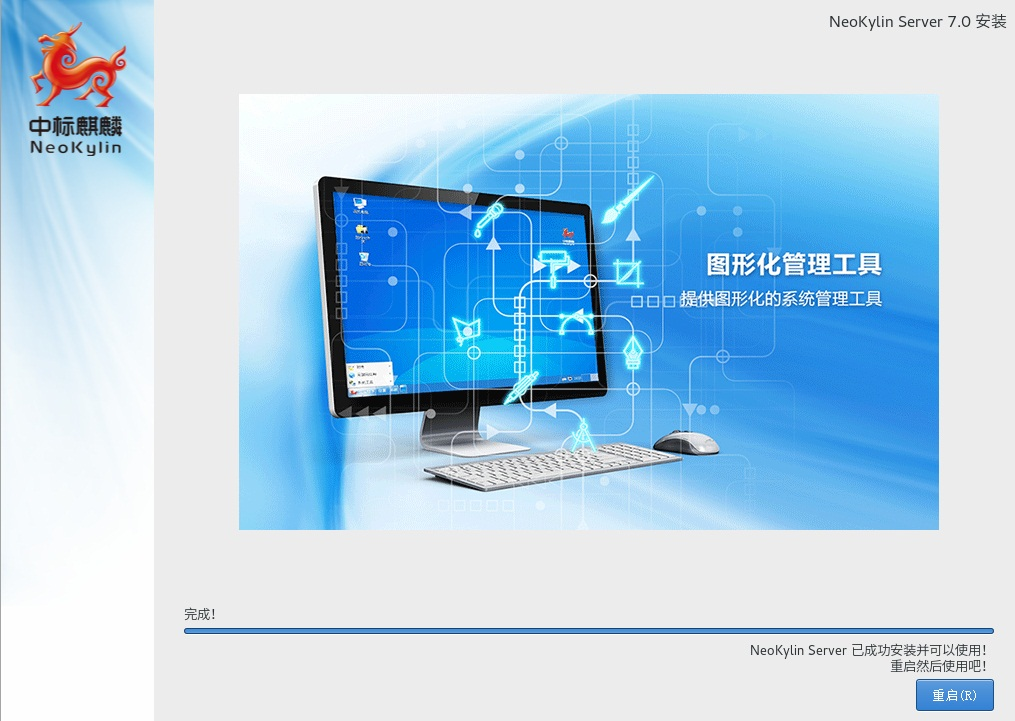
\includegraphics[width=10.5cm]{ns7/installation-progress-complete}
	\caption{安装完成}\label{fig:installation-progress-complete}
\end{figure}

点击\textbf{重启},即可体验中标麒麟服务器操作系统~V7.0~(~aarch~64~版)。

\end{document}